\section{Dataset Details}
\subsection{Stab Stereo Dataset}
\begin{frame}{Dataset}
    \begin{itemize}
        \begin{columns}
        \begin{column}{.4\textwidth}
        \item Data spec
        \begin{itemize}
            \item \textbf{EDM stabs\footnotemark}(original)
            \item 400ms, 44.1kHz, 16bit wav
        \end{itemize}
        \end{column}
        \begin{column}{.3\textwidth}
        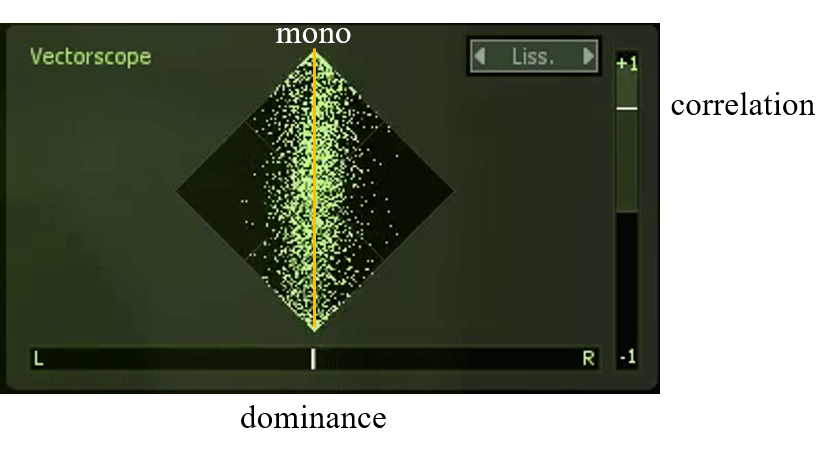
\includegraphics[width=1.5\linewidth]{Presentation/figures/dataset_vectorscope.png}
        \end{column}
        \end{columns}
        \bigskip
        \item Features
        \begin{itemize}
            \item Drastic stereo image changing over time
            \item Not too long (<1s)
            \item Almost atonal ($\because$ frequency modulated)
        \end{itemize}
    \end{itemize}
    \footnotetext[1]{Stab: A single staccato note or chord that adds dramatic punctuation to a composition.}
\end{frame}

\begin{frame}{Dataset}
    \begin{block}{Examples}
    \bigskip
    \begin{minipage}{.24\textwidth}
        \centering
        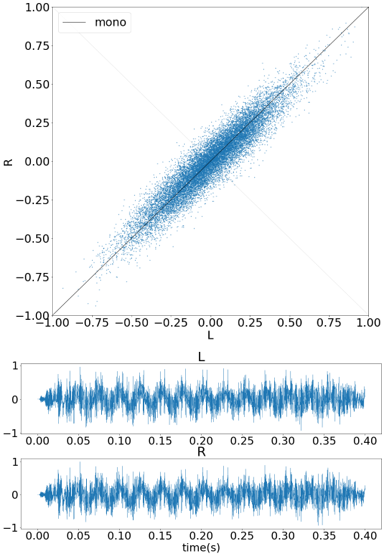
\includegraphics[width=0.9\linewidth]{Presentation/figures/dataset_example_1.png}
    \end{minipage}
    \begin{minipage}{.24\textwidth}
        \centering
        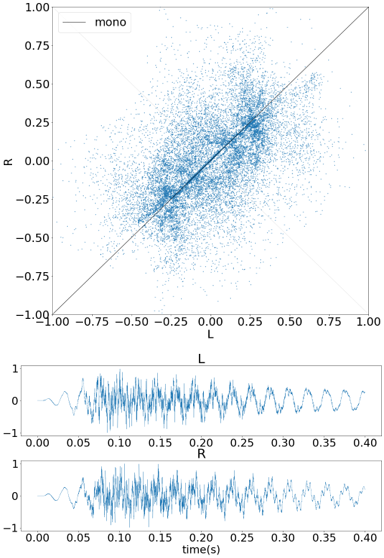
\includegraphics[width=0.9\linewidth]{Presentation/figures/dataset_example_2.png}
    \end{minipage}
    \begin{minipage}{.24\textwidth}
        \centering
        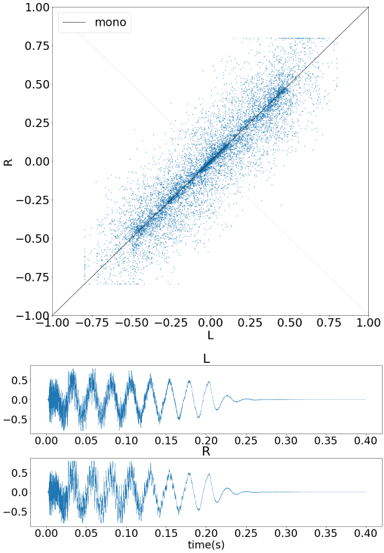
\includegraphics[width=0.9\linewidth]{Presentation/figures/dataset_example_3.png}
    \end{minipage}
    \begin{minipage}{.24\textwidth}
        \centering
        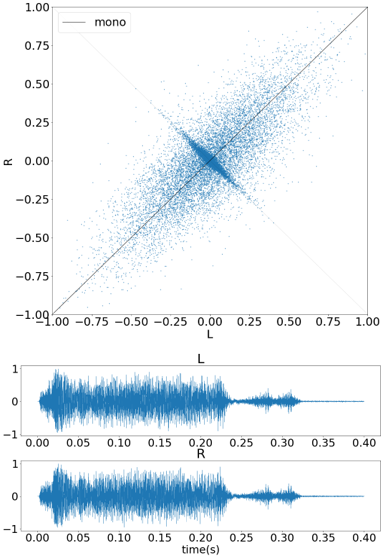
\includegraphics[width=0.9\linewidth]{Presentation/figures/dataset_example_5.png}
    \end{minipage}
    \end{block}
\end{frame}

\subsection{Augmentation}
\begin{frame}{Dataset}
    \begin{block}{Augmentation}
            \begin{itemize}
            \begin{columns}
            \begin{column}{.4\textwidth}
            \item L/R channel changing (x2)
            \item Time stretching w/o pitch shift (x3)
            \item FIR filtering (x4)
            \end{column}
            \begin{column}{.3\textwidth}
            \centering
            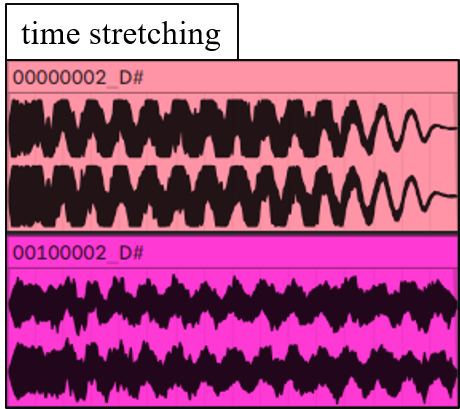
\includegraphics[width=1\linewidth]{Presentation/figures/augmentation1.png}
            \end{column}
            \end{columns}
        \end{itemize}
    \end{block}
        \begin{minipage}{.5\textwidth}
        \bigskip
        \bigskip
        \centering
        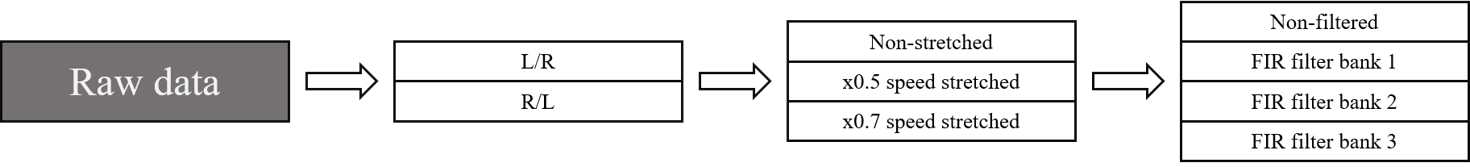
\includegraphics[width=2\linewidth]{Presentation/figures/augmentation2.png}
    \end{minipage}
\end{frame}

\subsection{Preprocessing}
\begin{frame}{Dataset}
    \begin{block}{Preprocessing}
        \begin{itemize}
            \item Converting original wav file to appropriate form (that network can consume directly) on-the-fly during training phase needs additional computing time and resources.
            \item We convert audio into mel spec + IF (Instantaneous Frequency)
        \end{itemize}
        \centering
        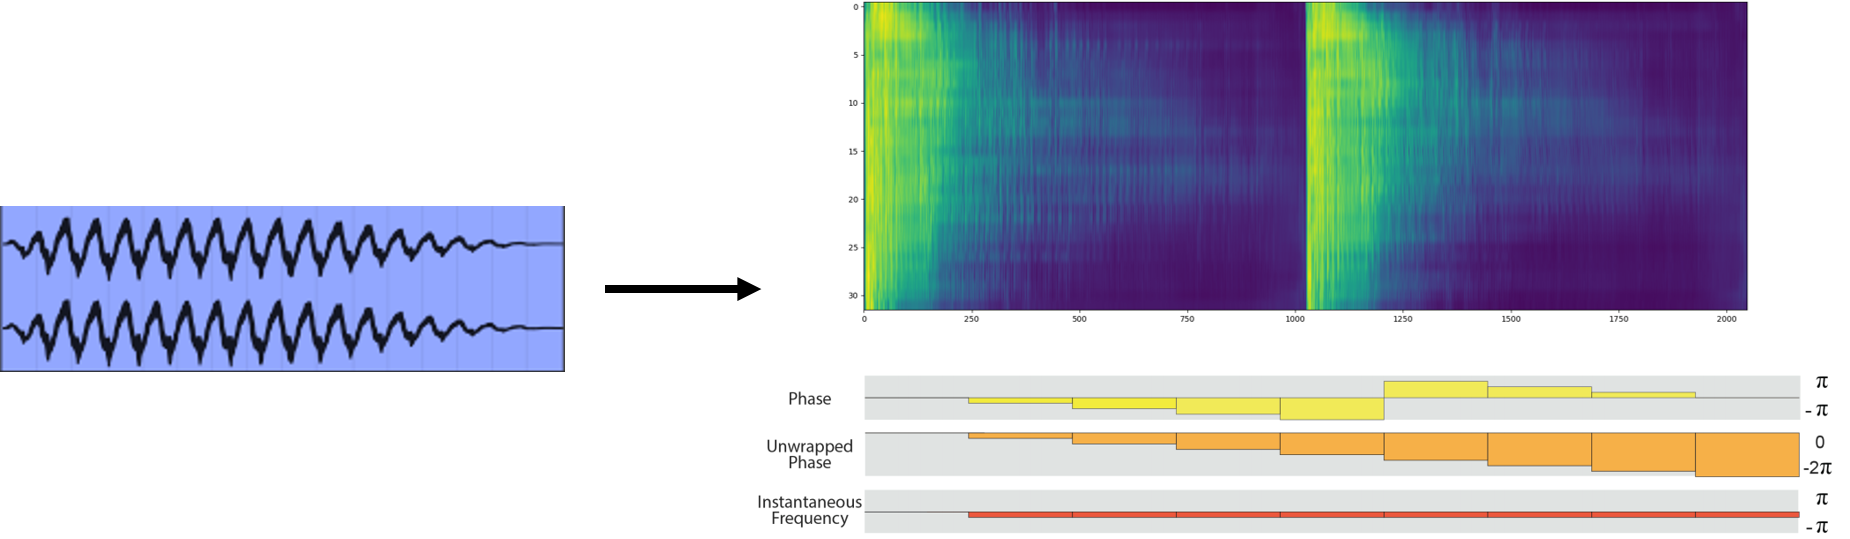
\includegraphics[scale=0.3]{Presentation/figures/dataset_preprocessing.png}
    \end{block}
\end{frame}